\section{Work Plan}
\label{sec:workplan}

\subsection{Phases}

\subsubsection{Planning phase}
In this phase, a lot of time went to researching development methodology,
different useful technologies (like \LaTeX{}, different frameworks, customer
needs, etc.), and deciding upon a template for the software architecture. This phase was scheduled 
for completion by September 16th. 

\subsubsection{Development}
This phase started as soon as the planning phase was completed and
approved by the customer. It included development of the different
applications and testing continuously. This phase was scheduled for completion by
November 15th.

\subsubsection{Report Writing}
This phase included writing the necessary documentation of the final code. A lot of work
was put into writing the report during the development phase. However, as the
report would be large, and we would need the time to make corrections
and add content. This phase was scheduled for completion by November 20th. 

\subsubsection{Planning of presentation}
Planning of the presentation was started after this report was completed. This phase was scheduled
for completion the day before the actual presentation November 22nd. 

\subsection{Activities}
\label{sec:activities}
We identified some big tasks that needed to be done during the project lifetime. These
tasks were essential to make the project a success. 

The identified tasks are:
\begin{itemize}
  \item Workshop
  \item Usability tests
  \item Integration tests
  \item Export applications and wrap up the source code
  \item Project presentation
  \item Final report correction
\end{itemize}

\subsection{Person-hours per activity and phase}
We planned the following person hours per phase. These numbers are based on the estimated project
effort according to the class staff, and how long we thought each phase would take. As the activities identified
in Section \ref{sec:activities} are activities ``baked into'' the different sprints during development, we have not included estimation for these 
(for instance, it is hard to know so early how many usability tests we need). Also, we would write the report continuously, 
and this is considered a subtask of both development and planning. For each sprint we planned to use 175 hours on development.
%TODO: begrunne 175 timer?
\begin{itemize}
  \item Development: 875 hours
  \item Planning: 425 hours
  \item Meetings: 125 hours
  \item Report completion: 30 hours
  \item Presentation planning: 30 hours
\end{itemize}

\subsection{Gantt Diagram}
Figure \ref{fig:gantt} shows the Gantt Diagram for the whole project period.
%TODO: write something about the gantt diagram
\begin{figure}
	\centering
		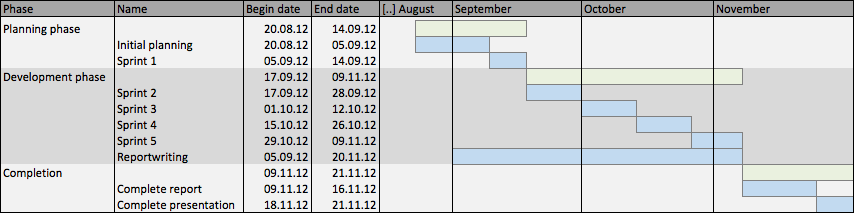
\includegraphics[width = 17.5 cm]{Pictures/ArchPictures/Gantt.png}
	\caption{Gantt project overview}
	\label{fig:gantt}
\end{figure}